% Created 2019-12-26 Thu 18:30
% Intended LaTeX compiler: pdflatex
\documentclass[11pt]{article}
\usepackage[utf8]{inputenc}
\usepackage[T1]{fontenc}
\usepackage{graphicx}
\usepackage{grffile}
\usepackage{longtable}
\usepackage{wrapfig}
\usepackage{rotating}
\usepackage[normalem]{ulem}
\usepackage{amsmath}
\usepackage{textcomp}
\usepackage{amssymb}
\usepackage{capt-of}
\usepackage{hyperref}
\author{Heitor Lourenço Werneck \\{\href{mailto:heitorwerneck@hotmail.com}{heitorwerneck@hotmail.com}}}
\usepackage[portuguese]{babel}
\usepackage{mathtools}
\usepackage[binary-units=true]{siunitx}
\usepackage[top=0.5cm,bottom=1.5cm,left=2cm,right=2cm]{geometry}
\usepackage{mdframed}
\usepackage{listings}
\usepackage[noend]{algpseudocode}
\usepackage{algorithm}
\usepackage{tikz}
\usepackage{xcolor}
\usepackage{colortbl}
\usepackage{graphicx,wrapfig,lipsum}
\RequirePackage{fancyvrb}
\DefineVerbatimEnvironment{verbatim}{Verbatim}{fontsize=\small}
\usepackage[font=small,labelfont=bf]{caption} % Required for specifying captions to tables and figures
\usepackage[subrefformat=parens]{subcaption}
\date{\today}
\title{Grafos\\\medskip
\large Trabalho Prático 1}
\hypersetup{
 pdfauthor={Heitor Lourenço Werneck},
 pdftitle={Grafos},
 pdfkeywords={},
 pdfsubject={},
 pdfcreator={Emacs 26.3 (Org mode 9.1.9)}, 
 pdflang={Portuguese}}
\begin{document}

\maketitle
\tableofcontents

\definecolor{bg}{rgb}{0.95,0.95,0.95}
\BeforeBeginEnvironment{minted}{\begin{mdframed}[backgroundcolor=bg]}
\AfterEndEnvironment{minted}{\end{mdframed}}
\numberwithin{equation}{section}
\algnewcommand{\IfThenElse}[3]{% \IfThenElse{<if>}{<then>}{<else>}
  \State \algorithmicif\ #1\ \algorithmicthen\ #2\ \algorithmicelse\ #3}

% Define block styles
\tikzstyle{decision} = [diamond, draw, fill=blue!20, 
    text width=4.5em, text badly centered, node distance=3cm, inner sep=0pt]
\tikzstyle{block} = [rectangle, draw, fill=blue!20, 
    text width=5em, text centered, rounded corners, minimum height=4em]
\tikzstyle{line} = [draw, -latex']
\tikzstyle{cloud} = [ellipse, draw, fill=red!20, 
    text width=5em, text centered, rounded corners, minimum height=2em]
%\tikzstyle{cloud} = [draw, ellipse,fill=red!20, node distance=3.5cm,
%    minimum height=2em]


\lstset{
  basicstyle=\ttfamily,
  columns=fullflexible,
  frame=single,
  breaklines=true,
  postbreak=\mbox{\textcolor{red}{$\hookrightarrow$}\space},
}
\newpage
\section{Introdução}
\label{sec:org2b7e11e}
Algoritmos de obtenção de menor caminho em grafos são muito utilizados em diversas áreas como por exemplo: recomendação de sistemas, mapas geográficos, redes de telefonia e em diversos outras áreas.

Em um problema de menor caminho é dado um grafo ponderado e direcionado \(G=(V,E)\), a função de ponderamento é definida como \(w: E \rightarrow \mathbb{N}\).cite:rayward-smith91\_introd\_to\_algor

O caminho com menor peso do vertice \(u\) até o \(v\) é \(\delta(u,v)\). O mesmo é definido como:

\(\delta(u,v)=\begin{cases}min\{w(p):u \leadsto^{p} v\} & \text{se existir um caminho de u para v} \\ \infty & \text{se não}\end{cases}\)

Esse trabalho tem por objetivo apresentar um algoritmo que solucione o problema de encontrar o caminho mínimo entre todos pares de vértices de um grafo \(G\) e também fazer análise de um grafo de uma rede real.
O algoritmo feito foi o Floyd-Warshall, o Bellman-Ford também foi feito porém foi utilizado somente para validação do Floyd-Warshall.


\section{Modelagem e Solução}
\label{sec:orge76cdb2}

Primeiramente é importante definir como será representado o grafo \(G\). A escolha foi uma matriz de adjacência por sua facilidade de manipulação e também por causa de seu acesso aos elementos ser de complexidade assintótica de tempo \(O(1)\), essa operação é realizada muitas vezes nos algoritmos logo essa complexidade será benéfica.

O grafo será representado como:

\begin{equation}
\begin{bmatrix}
 v_{11} & v_{12} & \cdots & v_{1j} \\
 v_{21} & v_{22} & \cdots & v_{2j} \\
 \vdots & \vdots & \ddots & \vdots \\
 v_{i1} & v_{i2} & \cdots & v_{ij} \\
\end{bmatrix}
\end{equation}

Com \(v_{ij} \in \{0(\text{Não tem aresta}),1(\text{Existe aresta})\}\) para \(i=1,...,|V| \land j=1,...,|V|\).

\subsection{Floyd-Warshall}
\label{sec:org03230c5}

O algoritmo ref:alg:floydwarshall descreve o funcionamento detalhadamente. Como é possivel ver pelos laços a complexidade assintótica de tempo é \(O(n^3)\). No final do algoritmo uma matriz de distâncias de todos pares de vértices é obtida.

\begin{algorithm}
\textbf{Input:} $G$
\textbf{Output:} $d$
\caption{Floyd-Warshall.}\label{alg:floydwarshall}
\begin{algorithmic}[1]
\Procedure{floyd\_warshall}{}
\State $d\gets copy(G)$
\For{$k = 1$ to $G.|V|$}
\For{$i = 1$ to $G.|V|$}
\For{$j = 1$ to $G.|V|$}
\If{$d[i,j]>d[i,k]+d[k,j]$}
\State $d[i,j]\gets d[i,k]+d[k,j]$
\EndIf
\EndFor
\EndFor
\EndFor
\State \Return $d$
\EndProcedure
\end{algorithmic}
\end{algorithm}

\section{Análise de Resultados}
\label{sec:org180bcbc}

A base de dados escolhida para ser feito a análise foi o \emph{Yelp Dataset Challenge} cite:WinNT. Dessa base de dados foi retirado os dados sobre as amizades dos usuários da cidade de Madison, esse grafo é não direcionado.

O grafo terá seus vértices como usuários e as arestas como relação de amizade entre usuários. Foi obtido um total de 1022 usuários(vértices) e 5078 amizades(arestas).

A densidade do grafo é de 0.0097329, ou seja, bem baixa. Isso mostra que pessoas são amigas de poucas pessoas.

O clique do grafo é 17, isso mostra que existe uma pequena comunidade de amizade no grafo.

Na figura ref:fig:graph mostra uma amostragem de 30 usuários do grafo.

\begin{figure}[htbp]
\centering
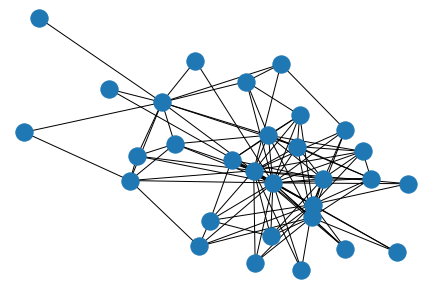
\includegraphics[width=.9\linewidth]{../graph.png}
\caption{\label{fig:graph}
Grafo da rede de usuários.}
\end{figure}

A partir desses dados inicias foi iniciado o processo de análise de localização dos vértices. Primeiro foi executado o algoritmo ref:alg:floydwarshall no grafo e foi obtido a matriz de distâncias.
Com essa matriz foi obtido o número mínimo, máximo e médio de cada linha. Não é necessário fazer para as colunas pois o grafo é não direcionado e o processo seria redundante.

\begin{equation}
\begin{bmatrix}
 0 & 2 & 1 & \text{min}=1,\text{média}=1.5,\text{max}=2 \\
 2 & 0 & 1 & \text{min}=1,\text{média}=1.5,\text{max}=2 \\
 1 & 1 & 0 & \text{min}=1,\text{média}=1,\text{max}=1 \\
\end{bmatrix}
\end{equation}

Um problema na análise desse grafo é que se existir um usuário com distância máxima infinito então todos outros também terão essa mesma distância máxima, que é o que aconteceu, logo não poderá se ter uma análise detalhada com base nesse aspecto. Porém para utilizar a informação de distância máxima foi considerado o maior valor sendo um valor menor que infinito se o mesmo existir, se não existir então o valor é infinito mesmo.

Como é possível ver na figura ref:fig:maxdist aproximadamente 80\% dos usuários possuem amizades, já os outros 20\% não possuem amizade. E de acordo com essa mesma figura existem mais pessoas com distâncias máximas menores em relação as outras, isso pode indicar que a maioria dos usuários não pertencem a redes grandes de amizade.

\begin{center}
\begin{figure}
\centering
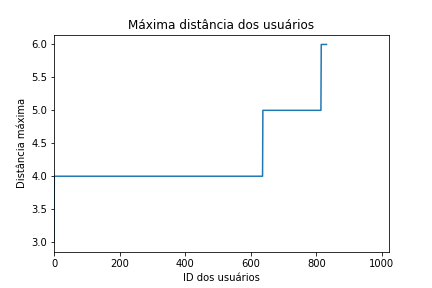
\includegraphics[width=7.5cm]{maxdist}
\caption{Distância máxima dos usuários.}\label{fig:maxdist}
\end{figure}
\end{center}

O problema no cálculo de distância máxima também se propaga para a distância média, logo para fazer a análise de distância média de um usuário foi desconsiderado os valores infinitos, porém se não existirem valores diferentes de infinito então a distância média é realmente infinito.

De acordo com a figura ref:fig:pmeandist e ref:fig:meandist pelo menos 50\% dos usuários tem um valor médio de distância bem constante.

Porém pela figura ref:fig:pmeandist do usuário 600 até o 800 há um crescimento considerável em relação a de 0 a 600. Isso pode mostrar uma relação de diferenciação grande de uma pequena parte dos usuários.

\begin{center}
\begin{figure}
\begin{subfigure}[b]{.49\linewidth}
\centering
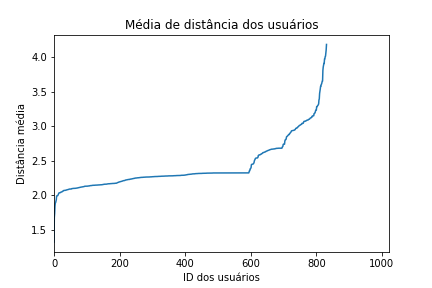
\includegraphics[width=7.5cm]{pmeandist}
\caption{}\label{fig:pmeandist}
\end{subfigure}
\begin{subfigure}[b]{.49\linewidth}
\centering
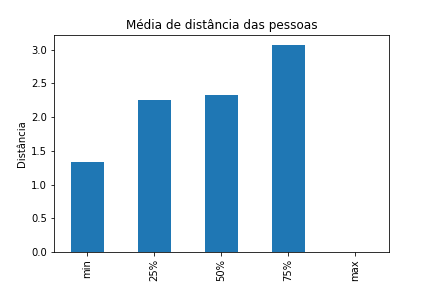
\includegraphics[width=7.5cm]{meandist}
\caption{}\label{fig:meandist}
\end{subfigure}
\caption{Distância média.}
\end{figure}
\end{center}

A distância mínima pode ser análisada tranquilamente sem os problemas anteriores mencionados.

Foi observado que 832 usuários possuem um valor mínimo menor que infinito, ou seja, eles possuem pelo menos uma amizade. Porém os outros 190 não possuem nenhuma amizade, isso também feito análisado de outra forma nos outros gráficos.

Isso indica que o \emph{dataset} escolhido possue 81.4\% de usuários com alguma amizade.


\section{Conclusão}
\label{sec:org990fc19}

Com o trabalho realizado foi possível fazer diversas observações sobre a base selecionada. A complexidade de tempo do algoritmo implementado na prática fez com que os resultados fossem produzidos com necessidade de muito tempo, o que corresponde a complexidade de \(O(n^3)\).

Foi possível obter diversas informações importantes sobre o grafo utilizando informação de distância, isso mostra sua importância na análise.

O \emph{dataset} análisado apresentou muitos usuários sem vértices ligando-os, isso mostra algo que pode ser recorrente em grafos de amizades em uma cidade.

Apesar dos problemas para fazer a análise as medidas tomadas para se solucionar os problemas se mostraram eficientes e foi possível prosseguir com a análise.

Então pode-se concluir que o trabalho foi um sucesso pois um algoritmo foi implementado para solucionar o problema de distância mínima e uma análise de uma base real foi feita.



bibliographystyle:plain
bibliography:doc.bib
\end{document}
